% Full title as you would like it to appear on the page
\chapter{Mapping the Statistics of the human B cell repertoire}
% Short title that appears in the header of pages within the chapter
\chaptermark{Repertoire \textit{in vivo}}

\section{Abstract}
B cells generate pathogen-specific antibodies, which provide adaptive protection against infectious microbes. Unlike most proteins, antibodies are not genetically encoded at birth. Rather, they are stochastically generated and then modified in evolutionary processes acting on the B cell populations within an individual. These populations clonally expand, migrate, and home to long-term niches throughout the body, but the dynamics of differentiation, proliferation, and migration patterns in the human immune system remain mostly inferred from mouse studies. To address this, we sequenced the B cell receptors (BCRs) and transcriptomes at the single-cell level in multiple immune-rich tissues from six individuals. These paired data enabled us to examine the phenotypic patterns of expansion, migration, and differentiation of related B cells (lineages). While most BCRs are detected in just a single tissue, we observed B cells with identical BCRs in multiple tissues. These cells differed from other subsets. They had often cycled recently and had more hypermutated BCRs than cells confined to a single tissue. Using phylogenetic approaches, we discovered that lineages often co-localize within the same tissue. However, when lineages reach a threshold size in the peripheral blood and secondary lymphatic organs (SLOs), their members are likely to be found in other tissues. This indicates that cellular migration from blood and SLOs is a probabilistic process in which cross-tissue sharing occurs when lineages attain sufficient size. Furthermore, we identified a hierarchy in migration patterns between tissues, with the spleen as the primary destination for hypermutated B cells and the bone marrow as the final location. Notably, the bone marrow had the largest fraction of private lineages compared to other examined tissues, consistent with its role as a terminal destination for plasma cells. Collectively, our findings elucidate the evolutionary landscape of B cell populations across tissues and show that the peripheral blood provides limited insights into the dynamics and composition of the human B cell repertoire.

\section{Introduction}
 Antibodies are developed by the immune system in response to pathogens and  provide protection to an individual in future exposures.  They are genetically encoded in B cells, which can remain alive throughout the lifetime of the individual\cite{slifka1998humoral}. These B cells provide long-term immune protection against previously encountered pathogens, as well as the capacity to rapidly respond to similar pathogens. During immune responses, clonal populations of B cells compete to receive proliferation and differentiation signals which direct them to become short or long-lived antibody secreting cells or memory B cells. 

Previous studies have uncovered much about the dynamics of this process in mice\cite{victora2022germinal},  and much is known about the characteristics of different B cell populations in humans\cite{halliley2015long, glass2020integrated, tarlinton2023making}, however, we still know very little about the statistics of B cell differentiation in healthy humans. As a result, it remains unclear, for instance, how the memory B cell subset in humans is related to the antibody secreting cell subset, or how the different types of antibody secreting cells are related to one another\cite{tarlinton2023making}. 

In principle, questions about the genetic relationships of different B cells can be resolved by sequencing the B cell receptor (BCR) of B cells in different subsets and investigating the phylogenetic relationships of the cells in these groups\cite{ellebedy2016defining,briney2019commonality,phad_lanza_2022clonal, horns2016lineage}. However, most effector B cells in humans reside in tissues that are difficult to sample, while previous BCR sequencing studies on healthy humans have largely been carried out on B cells sampled from the peripheral blood. To address this gap, several recent studies have surveyed B cell populations resident in other tissues\cite{glass2020integrated, tabula2022tabula, dominguez2022cross}.  These studies reveal that B cells living in other tissues are exist in a range of diverse effector states, which often differ from the B cell subsets that have been described in mice\cite{glass2020integrated, dominguez2022cross}. However, limitations in either the number of sampled B cells in these studies or the availability of the corresponding BCR sequences have made it impossible to use these studies to answer questions about the relationships between B cells in different tissues and states. Other work\cite{meng2017atlas, yang2021shared} revealed complex patterns of genetic relationships between the B cell populations sampled from a wide range of human organs by sequencing BCRs. However, these data lacked phenotypic information and single-cell resolution, making it difficult to interpret these relationships in light of the underlying cellular processes of differentiation and migration. 

Here we use a combination of single-cell transcriptome and BCR sequencing to simultaneously measure the phenotypic and genetic relationships of B cells resident in a range of immune-rich tissues in six healthy individuals. Our simultaneous measurement of the transcriptome and BCR allows us to associate BCRs with a B cell's functional state and to jointly investigate the patterns of B cell migration and differentiation between human organs.
\section{Results}

\subsection{The distribution of B cells in lymphatic tissues at rest}
 We obtained B cells from the vertebral bodies, supradiaphragmatic and mesenteric lymph nodes, spleen, and blood of 6 organ donors with no clinical history of cancer, immune disease, or active infectious disease at the time of death (Figure \ref{fig:study-overview}\textbf{a}, \ref{tab:donor-metadata}, methods). We used high-throughput droplet-based single cell RNA-sequencing to analyze the transcriptomes and BCRs of over 200 thousand single B cells. To increase the depth of BCR sampling, and to provide replication of the sampling and measurement process, we used the same platform to sequence only the BCRs of an additional 400 thousand B cells. 

Overall, we observe a remarkably quiescent immune system, with very few activated B cells detected in all donors (Figure \ref{fig:study-overview}\textbf{b}). A small fraction of all B cells (1-6\% per donor) appear to be actively proliferating as evidenced by the expression of M-phase markers such as MKI67 (methods, \ref{ED:cycling}).  Proliferating cells predominantly have an antibody secreting cell (ASC) phenotype, though we sampled a small number of proliferating germinal center B cells, as well as a small fraction of age-associated B cells (ABCs) that appear to be actively dividing (Figure \ref{ED:cycling}\textbf{d}).

\subsection{Distribution of cell types among organs}
The fraction of cycling B cells and B cell types in general was similar across tissues. However, the SLOs had a much larger relative abundance of memory B cells, which was offset by a smaller relative abundance of naive B cells (Figure \ref{fig:study-overview}\textbf{c}). Similarly, the the bone marrow had a much larger relative abundance of antibody secreting cells, offset by a smaller relative abundance of memory B cells. Cells with a germinal center-like phenotype were almost exclusively detected in SLOs, and at relative abundances near 1 in 1000, showing very limited ongoing systemic immune responses in all donors  (Figure \ref{fig:study-overview}\textbf{c}). Though the distribution of hypermutation levels in all  non-naive cell types was broad, we observed large differences in median hypermutation levels between antibody secreting cells and memory B cells, with ASC having median 10 additional mutations compared memory B cells in the same tissue\ref{fig:asc-overview}\textbf{d},\ref{ED:memoryb-overview}\textbf{d}).   
\begin{figure}
    \centering
    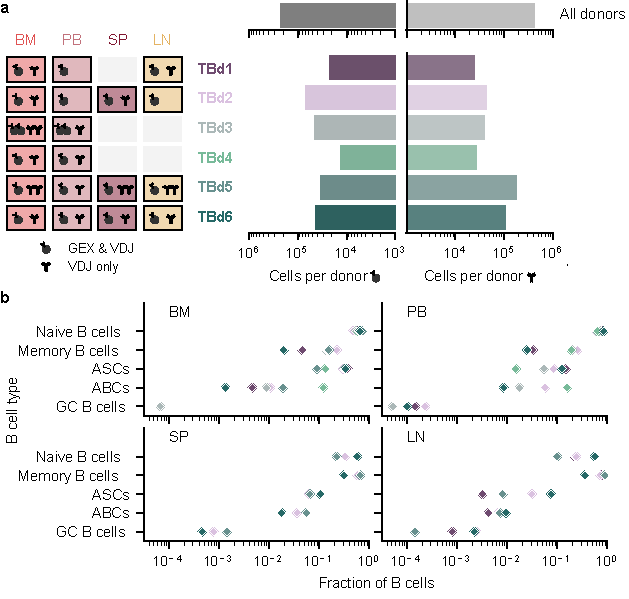
\includegraphics[width=10cm]{figs/Tabula_Bursa/Figure1_ab_antibody_version.pdf}

    \caption[\textit{In vivo} study overview]{Heterogeneity in antibody secreting cells (ASCs). (a) Low-dimensional (UMAP) representation of transcriptional heterogeneity in ASCs. Celltypist labels (top), and transcriptome-derived labels (bottom). Inset shows UMAP representation when cell-cycle associated genes are removed. (b) Genes distinguishing between the subtypes of ASCs, where the top half of the plot shows canonical genes often used for flow cytometry and the bottom shows the data-derived, transcriptionally detected genes which distinguish the subtypes. (c) The relative fractional abundance of ASC subtypes in different tissues averaged across all donors. (d) The distributions of  hypermutation levels (d),  and constant region usage (e) of the ASC subtypes}
    \label{fig:study-overview}
\end{figure}
\begin{table}[t]
\centering
\begin{tabular}{|c|c|c|c|c|}
\hline
\textbf{Donor} & \textbf{Age} & \textbf{Sex} & \textbf{Ethnicity} & \textbf{Cause of Death} \\
\hline
TBd1 & 46 & F & Asian/Japanese & Cerebrovascular stroke \\
TBd2 & 35 & M & American Indian or Alaska Native & Anoxia \\
TBd3 & 25 & F & Hispanic/Latino & Head Trauma \\
TBd4 & 43 & F & Hispanic/Latino & Anoxia \\
TBd5 & 45 & F & Asian / Filipino & Cerebrovascular stroke  \\
TBd6 & 60 & M & Asian / Filipino & Anoxia, spontaneous cardiac arrest \\
TBd7 & 42 & M & Other Race & NA \\
\hline
\end{tabular}
    \caption[Table of Donor Metadata]{Demographic characteristics of  donors}

    \label{tab:donor-metadata}
\end{table}

\subsection{Phenotypic variability among memory and antibody secreting cells}



Initially, we automatically annotated the B cell types using an algorithm called \verb|celltypist|\cite{dominguez2022cross}. However, our data reveal substantial additional phenotypic variability within non-naive B cell subsets (Figures \ref{fig:asc-overview}, \ref{ED:memoryb-overview}). Among antibody secreting cells (ASC) (Figure \ref{fig:asc-overview}\textbf{a}), the variability was consistent with a prevailing understanding these cells have substantial phenotypic variation in mice and human (\cite{tarlinton2023making, halliley2015long}). 

\begin{figure}
    \centering
    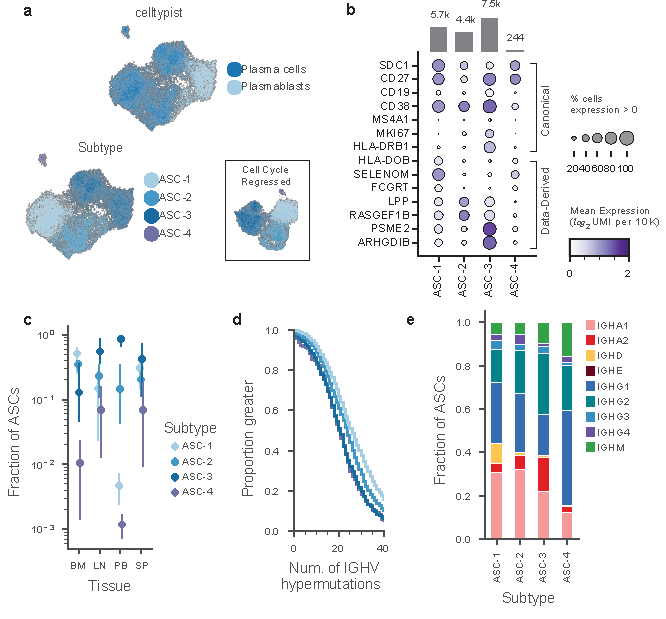
\includegraphics[width=12cm]{figs/Tabula_Bursa/Figure2_ASC_subtypes.pdf}

    \caption[Heterogeneity in antibody secreting cells (ASCs)]{ (a) Low-dimensional (UMAP) representation of transcriptional heterogeneity in ASCs. Celltypist labels (top), and transcriptome-derived labels (bottom). Inset shows UMAP representation when cell-cycle associated genes are removed. (b) Genes distinguishing between the subtypes of ASCs, where the top half of the plot shows canonical genes often used for flow cytometry and the bottom shows the data-derived, transcriptionally detected genes which distinguish the subtypes. (c) The relative fractional abundance of ASC subtypes in different tissues averaged across all donors. (d) The distributions of  hypermutation levels (d),  and constant region usage (e) of the ASC subtypes}
    \label{fig:asc-overview}
\end{figure}
There were four distinguishable types of ASC, which we label ASC-1 through ASC-4. A substantial fraction of ASC-3 were proliferating, had a gene expression signature that closely resembles previous descriptions of plasmablasts. For example, they expressed HLA molecules higher than other subsets (Figure \ref{fig:asc-overview}\textbf{b})\cite{sanz2019challenges}. Notably, nearly half of ASC-3 have no detectable M-phase markers, but have otherwise indistinguishable gene expression profiles from cycling ASC-3, suggesting that these cells have recently stopped cycling (Figure \ref{fig:asc-overview}\textbf{a}). Specifically, regressing the expression of the proliferation marker MKI67 collapses the distinction between the gene expression space of cycling and non-cycling ASC-3 (Figure \ref{fig:asc-overview}\textbf{a} inset). The other types of ASCs appeared non-proliferative, were commonly found outside the peripheral blood, and had gene expression consistent with long-lived plasma cell subtypes\cite{sanz2019challenges}(Figure \ref{fig:asc-overview}\textbf{b}). In particular, ASC-1 are primarily resident in the bone marrow and have the canonical markers of long-lived plasma cells (\cite{halliley2015long} (Figure \ref{fig:asc-overview}\textbf{b,c}). ASC-4 is strongly enriched in the SLOs, but transcriptionally similar to ASC-1. We performed differential expression analysis on these subsets of ASCs and found that ASC-1 and ASC-4 had higher expression of FCGRT (FcRN), SELENOM, and HLA-DO than other subsets. (Figure \ref{fig:asc-overview}\textbf{b}. SELENOM may participate in disulfide bond creation, but has no described role in antibody secretion or plasma cell longevity. We detected plasma cells of all isotypes, including a small proportion of plasma cells which were IGHD+ and heavily hypermutated compared to other isotypes (Figure \ref{fig:asc-overview}\textbf{d}). With respect to the memory B cells, we characterized their phenotypic profiles in a similar manner (Figure \ref{ED:memoryb-overview}) and found results generally consistent with a multi-omic characterization of B cells made by\cite{glass2020integrated}.

\subsection{VDJ sequencing reveals sharing of a subset of expanded clones}
\begin{figure}
    \centering
    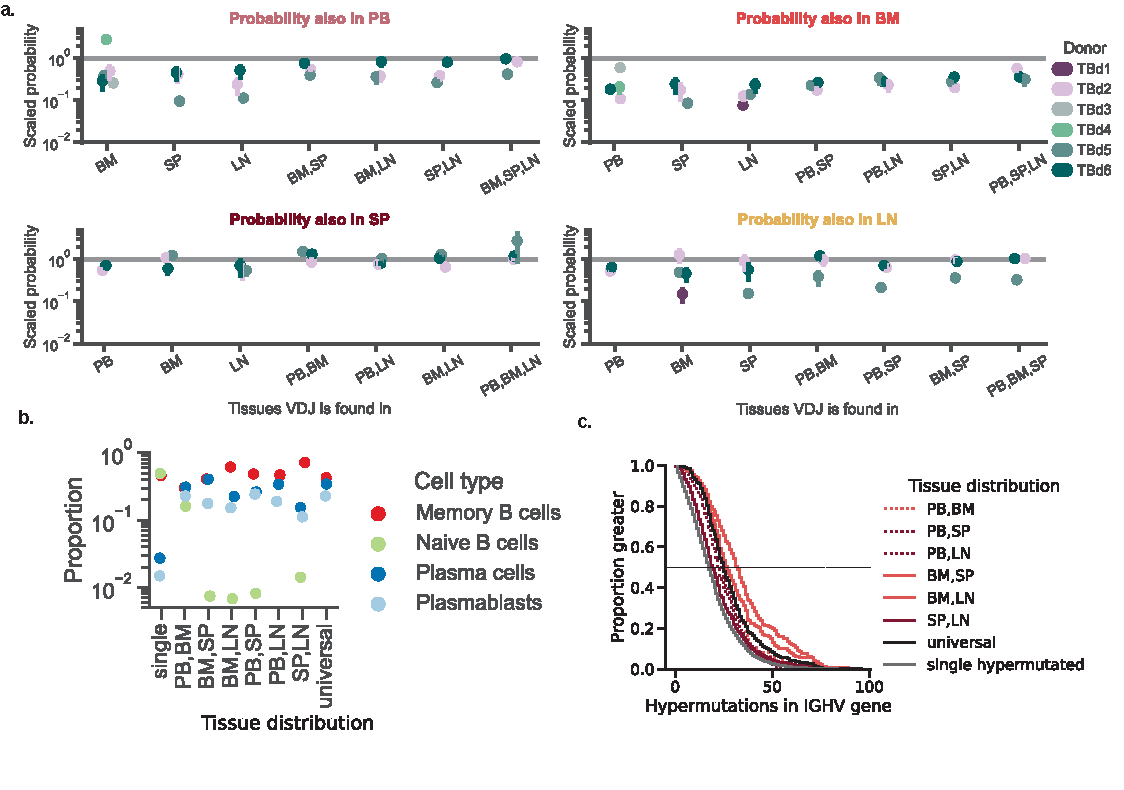
\includegraphics[width=10cm, keepaspectratio]{figs/Tabula_Bursa/Figure3_revised.pdf}
    \caption[Characteristics of clonally expanded B cells.]{ (a) Probability that a B cell is found in an additional tissue, given it is found to be expanded in one or more other tissues. (b) Fractional abundances, and (c) the distribution of hypermutation levels of B cells as a function of the tissues their heavy chain antibody sequences were found in.}
    \label{fig:clonally-expanded-B-cells}
\end{figure}
 In all samples, we sequenced the transcripts encoding for the heavy and light chains of the BCR, which we used to reveal the clonal relationships between B cells residing in different organs (methods, SI). We find that the probability of sampling identical nucleotide heavy chain sequences in different donors is vanishingly rare: after identifying and removing rare cross-contamination events (SI), we find only 5 of more than 600 thousand unique VDJs shared between donors, \ref{ED:multidonor-vdjs}. This observation is consistent with earlier work which showed convergent VDJ recombination is an extremely rare event (\cite{mora2019many, briney2019commonality}). Thus, we interpret the nucleotide sequence of the heavy chain variable region as a unique clonal identifier of B cells (SI). 
 
\begin{figure}
    \centering
    \includegraphics[width=10cm]{figs/Tabula_Bursa/ED_donor_sharing.pdf}
    \caption[Characteristics of  VDJ sequences found in multiple donors.]{(a) Number of unique nucleotide VDJ sequences as a function of the donors they were found in. (b) Distribution of the number of hypermutations in the templated portion of the IGHV gene as a function of the number of donors a VDJ sequence was found in. (c) Number of shared "clonotypes" in our data, where a clonotype is taken to be a sequence with an identical germline V gene, J gene, and CDR3 amino acid sequence. (d) Recombination probabilities for the CDR3 nucleotide sequence as a function of the number of donors the CDR3 was found in. Green dashes denote the CDR3's associated with the VDJ sequences shared between multiple donors. (e) Number of shared CDR3s in our data compared to the number expected under given the overall distribution of recombination probabilities shown in (d). The two models are described in detail in the SI.}
    \label{ED:multidonor-vdjs}
\end{figure}

Consistent with the variation in cell states revealed by our gene expression data, the characteristics of the VDJs differ between the tissues. In all donors, the peripheral blood and the bone marrow contain a substantial fraction of unhypermutated VDJs, while the bone marrow is also the site with the most heavily hypermutated sequences (\textbf{still missing, decide where to place}). Consistent with the relative paucity of naive B cells in the SLOs, VDJs sampled from these tissues predominantly contain hypermutations. 

Because we have single cell information, we are able to find that clonal expansion without hypermutation is a relatively common event: in all samples, about 1 in 100 of all unique VDJ sequences are identical in multiple cells. Though evidence of clonal expansion can be found among cells of all types, it is particularly prominent among antibody secreting cells, especially Type 3 ASCs, whether or not they are actively expressing M-phase associated genes (\textbf{panel still missing, decide where to place}). 

Next, we quantified the rates of clonally expanded VDJ sharing between tissues. To account for limited sampling, we derive a scaled probability estimate that makes use of technical replicates of tissue samples (SI, \ref{fig:clonally-expanded-B-cells}). VDJs expanded in one tissue are found in others with probabilities often exceeding 0.1. The patterns of relative sharing suggest a hierarchy between the lymphatic organs organs: the probability that a VDJ expanded in a given organ is also present in the spleen is often indistinguishable from 100\%, whereas the probability that it is found in the peripheral blood or in the bone marrow is typically lower. Finally, the probability of encountering a VDJ in any given tissue increases with the number of other tissues it has been seen in (Figure \ref{fig:clonally-expanded-B-cells}\textbf{a}). Multi-tissue-VDJs were enriched for the antibody secreting cell and memory B cell phenotypes  (Figure \ref{fig:clonally-expanded-B-cells}\textbf{b}). Furthermore, these VDJs are more strongly hypermutated than the comparable VDJs from ASCs and memory B cells restricted to a single tissue (Figure \ref{fig:clonally-expanded-B-cells}\textbf{c}). Finally, our data do not exclude the possibility that all cycling cells are shared between at least a pair of organs but we emphasize that not all cells that are shared are cycling: cells without M-phase markers account for a substantial fraction of all shared cells (Figure \ref{ED:cycling}).


\subsection{The distribution of related B cells among lymphatic tissues}
\begin{figure}
    \centering
    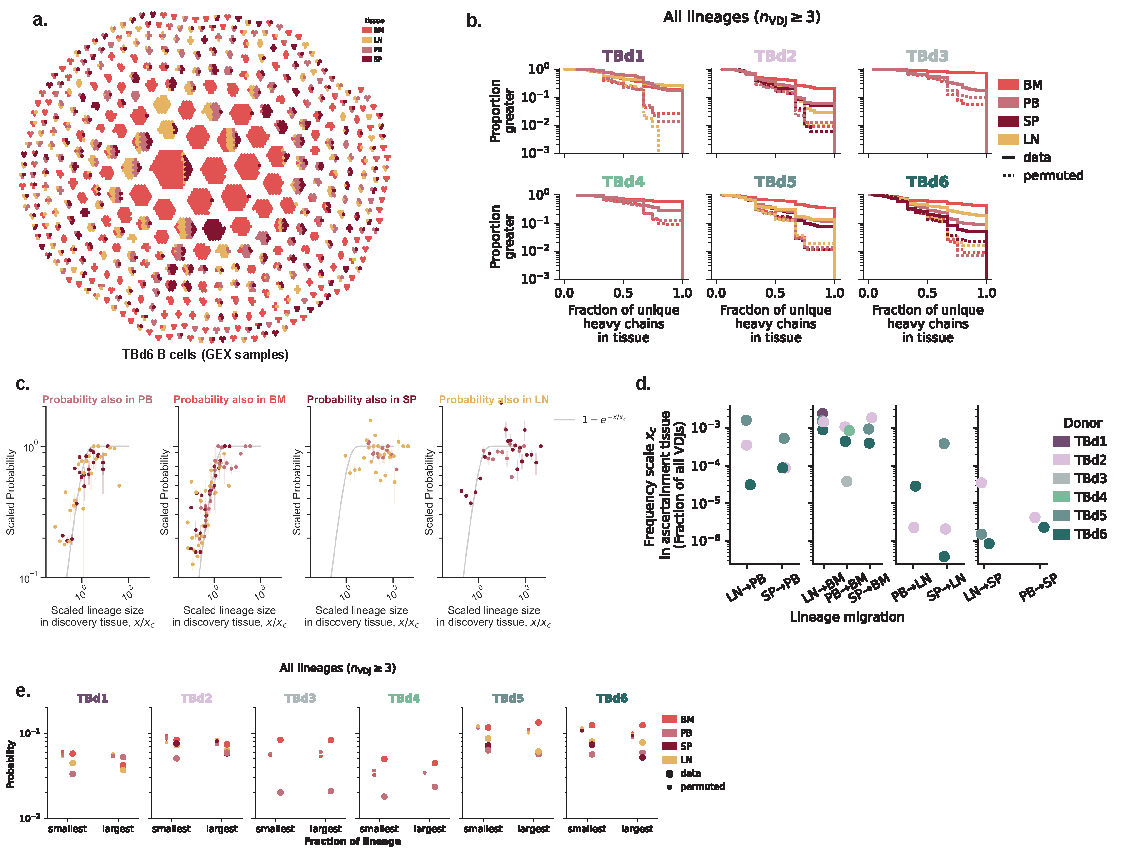
\includegraphics[width=10cm, keepaspectratio]{figs/Tabula_Bursa/Figure4_revised.pdf}
    \caption[Tissue distribution of phylogenetically related B cell, or lineages.]{(a) A representation of the tissue composition of lineages. Each hexagon denotes a cell, and each connected group of hexagons represents a lineage. Cells are colored by the tissue they were sampled in. Each tissue has been down-sampled to the same overall number of cells. (b) The distribution of the fraction of unique VDJs in the lineage found in a certain tissue. Dotted lines denote the distributions obtained after a random permutation of the tissue labels among the sampled cells.  (c) The probability that a lineage is discovered in a tissue, as a function of the total size of that lineage in another, ascertainment, tissue. Points are colored by ascertainment tissue, and each panel corresponds to a different discovery tissue. Size represents the total fraction of unique heavy chain sequences attributable to the lineage, and is scaled by a single parameter, the critical size $x_c$. (d) The critical size of a lineage in the ascertainment tissue used to scale lineage sizes in (c). (e) The probability that a tissue either contains the smallest or largest number of unique VDJ sequences in a lineage (relative to all other tissues). Large points are derived from the data, and small points represent a random permutation of the tissue labels among the sampled cells.}
    \label{fig:lineage-distribution}
\end{figure}

 B cells descended from the same VDJ recombination event carry a unique genetic recombination signature that we used to group B cells into clonal lineages. A striking feature of the distribution of lineages among the sampled tissues is the tendency for related cells to co-localize within the same tissue. (Figure \ref{fig:lineage-distribution}\textbf{a,b}). This co-localization is seen in all tissues and in all donors except TBd1, and is particularly strong in the case of the bone marrow. (Figure \ref{fig:lineage-distribution}\textbf{b}).  However, we detect abundant sharing of large lineages between the sampled organs. This sharing follows a relatively simple pattern: conditional on sampling a lineage in the peripheral blood, the spleen, or a lymph node, the probability that lineage is present in a second tissue increases exponentially with its size (Figure \ref{fig:lineage-distribution}\textbf{c}). Lineages in the bone marrow deviate from this scaling: large lineages in the bone marrow are no more likely to be present in another tissue than smaller lineages detected in the bone marrow. This suggests that migration of B cells out of the peripheral blood, spleen, or bone marrow is governed by a relatively simple probabilistic process, where a small, but constant probability exists that a cell residing in one of these three tissues migrates to a new tissue. In contrast, we find little evidence of such a process in the bone marrow, which tends to be the most exclusive tissue, as evidenced by the fact that it is the tissue most likely to be both the minority and the majority location for a B cell lineage (Figure \ref{fig:lineage-distribution}\textbf{e}).

By examining the size at which lineages sampled in these three tissues are guaranteed to be seen in another tissue, we uncover a hierarchy in the relative amounts of sharing between tissues. Lineages of relatively small size in the peripheral blood could be detected in the lymph nodes and spleen; lineages needed to reach a larger relative fraction in the spleen and lymph nodes to be also found in the blood, and an even higher size threshold was necessary for migration into the bone marrow (Figure \ref{fig:lineage-distribution}\textbf{d}). Overall, these patterns are consistent with the patterns of sharing of identical VDJs across tissues and suggest that the spleen in particular, and the lymph nodes to a lesser extent, may act as a first repository of B cells that have experienced affinity maturation, whereas the circulation of mature B cells in the peripheral blood, and finally localization in the bone marrow are less probable events.

%To understand the relative imbalance of lineage sharing amongst tissues, we calculated the number of times a specific tissue accounted for the smallest fraction and largest fraction of members in a lineage. Across all donors, these statistics deviated from a permuted null-expection for the bone marrow. 

\subsection{The distribution of tissues and cell types among groups of related cells}
 Overall, these results and the implied fractional abundance scales suggest that B cell migration is a relatively rare event relative to hypermutation. Given the differences in hypermutation rates of the same celltype in different tissues, we were interested in whether localization to certain tissues (e.g. the bone marrow) tended to occur deeper in lineage phylogenies. 

\begin{figure}
    \centering
    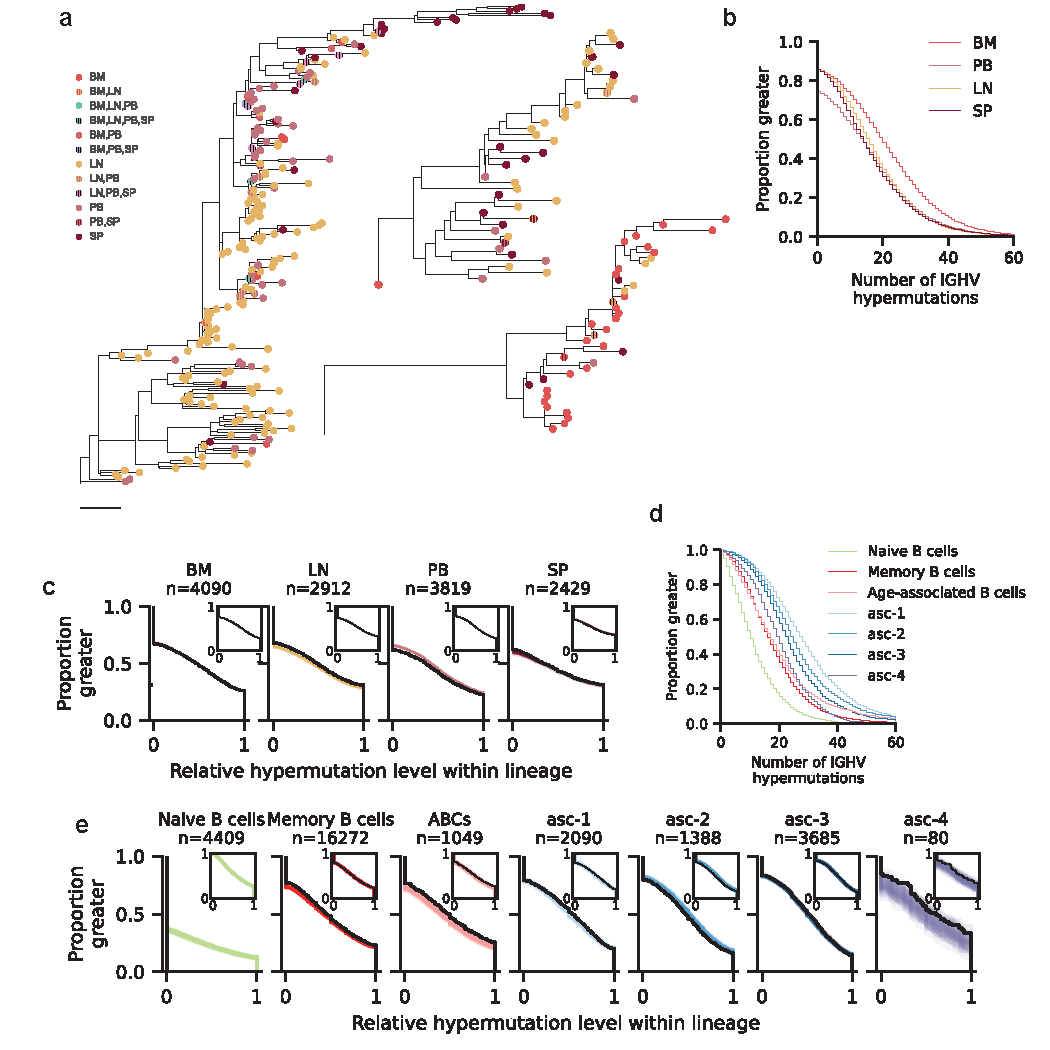
\includegraphics[width=10cm, keepaspectratio]{figs/Tabula_Bursa/Figure5_revised.pdf}
    \caption[Relationships between related cells.]{(a) Templated V gene trees depicting the relationships of B cells localized in different tissues in 3 example lineages from TBd6. Trees are rooted on the inferred germline V sequence. Leaves correspond to unique templated V sequences and are colored by localization. (b) The distribution of hypermutation levels of B cells belonging to lineages with membership in the indicated tissues. (c) Relative hypermutation levels of B cells within a lineage. In each panel, black lines denote the observed distribution in the data and the colored lines denote the 99\% confidence interval obtained by permuting tissue labels within lineages. On each panel, $n$ indicates the number of lineages among which the permutation was performed. Insets show the distributions with all cells with no templated V mutations excluded.  (d) The distribution of hypermutation levels of B cells belonging to lineages with any members in the indicated B cell subsets. (e) Same as (c), but for B cell subsets, rather than tissues. }

\label{fig:phylogenetic-relationships}
    
\end{figure}

This would cohere with the idea that affinity maturation occurs in other tissues such as the spleen or the lymph nodes before migration to the bone marrow. To investigate this, we compared the hypermutation level of cells residing in different tissues within lineages (Figure \ref{fig:phylogenetic-relationships}). Notably, the overall level of hypermutation varies not only between cells residing in different tissues, but also between their relatives: B cells in lineages with any members in the bone marrow are for instance also more hypermutated than comparable cells from the same tissue, even if they may not themselves reside in the bone marrow (Figure \ref{fig:phylogenetic-relationships}\textbf{b}). However, within lineages, cells located in different tissues were almost entirely uniformly distributed (Figure \ref{fig:phylogenetic-relationships}\textbf{c}), and are limited to the differential localization of naive B cells in different tissues. Once cells with no evidence of hypermutation in the templated V sequence are excluded, there remain no statistically significant differences between the measured distributions of hypermutation levels of related cells residing in different tissues (Figure \ref{fig:phylogenetic-relationships}\textbf{c}, insets).  An analogous observation can be made regarding the hypermutation levels of cells in different functional states. Despite systematic differences in the hypermutation levels of  different B cell subsets and their relatives (Figure \ref{fig:phylogenetic-relationships}\textbf{d}), within lineages, we cannot detect differences in the level of hypermutation between related B cells in different functional states (Figure \ref{fig:phylogenetic-relationships}\textbf{e}). This suggests that both changes in localization and differentiation (i.e. into Memory and ASCs) occur uniformly throughout an immune response, and is likely a history-dependent event, consistent with some recent experimental results on the pace of LLPC formation in mice. 


\section{Conclusions}
Our comprehensive study of the B cell repertoire across multiple immune-rich tissues provides a clear statistical description of human B cell differentiation. We found the B cell system remains largely quiescent in the absence of active infection. This is surprising given we sampled organs from donors who had recently received COVID mRNA vaccines. Studies of vaccination have shown germinal centre reactions that last for months in response to these vaccines\cite{turner2021sars}, suggesting these ongoing reactions are quite localized. Our unbiased sequencing approach allowed us to identify four subtypes of ASCs and six subtypes of memory B cells. These types had distinct hypermutation profiles and constant region gene usage, indicating distinct cellular histories and probabilities of differentiation into these states. Our analysis of shared sequences between donors revealed clonotypes shared between healthy individuals were uncommon and no more probable than expected by random chance. This indicates in the absence of chronic viral infection\cite{setliff2018multi}, convergent evolution does not meaningfully shape the healthy immune repertoire. This remains true even in the spleen and supradiaphragmatic lymph nodes, where B cells are thought to frequently encounter the most common microbial antigens.   

The breadth and depth of our data allowed the first statistical analysis of lineage relationships between the diverse phenotypes and sites of B cell populations. Across all tissues except the bone marrow, we found that lineage size can predict whether the lineage will appear in another tissue. Furthermore, our analysis showed that any differentiated cell phenotype has a uniform probability of creation at any point in a lineage structure. This is is line with mouse work which shows long-lived plasma cells continuously populate the bone marrow during an immune response (ref). We found that amongst all cell types, cycling ASCs, are the most likely to be found in multiple tissues. This finding may cohere with data showing plasmablasts in healthy donors appear to derive almost exclusively from memory recall\cite{phad_lanza_2022clonal}. Those authors advanced an idea that bystander activation may be a mechanism of homeostatic immune memory maintenance in the absence of re-exposure to specific pathogens. Given cycling cells are most likely to also migrate, it is possible that cycling and migration are linked components of an antigen-independent homeostatic maintenance program for B cell memory. Indeed, the cycling ASCs were least likely amongst ASCs to express CD138 (SDC1), which is thought to help cells attach to the extracellular matrix and establish residence. We found the bone marrow to be the most private tissue, suggesting it is most difficult tissue arrive in, but that cells which do arrive may survive longer than other members of their lineage which had dispersed to other tissues.  
A goalpost for future studies is to produce recombinant antibodies for lineages of interest and determine their binding properties. Of particular interest are antibodies from large multi-tissue lineages, that appear to have been selected\cite{neher2014predicting} and those from the IGHD+ plasma cells, which were deeply hypermutated and almost exclusively found in the bone marrow.
In summary, our study provides a robust foundation for future research into B cell biology. By mapping the phenotypic and antibody diversity of B cells across multiple tissues, we provide valuable insights into the dynamics and composition of the human B cell repertoire. The data generated in this study should prove crucial in advancing our understanding of human B cell differentiation.


\begin{figure}
    \centering
    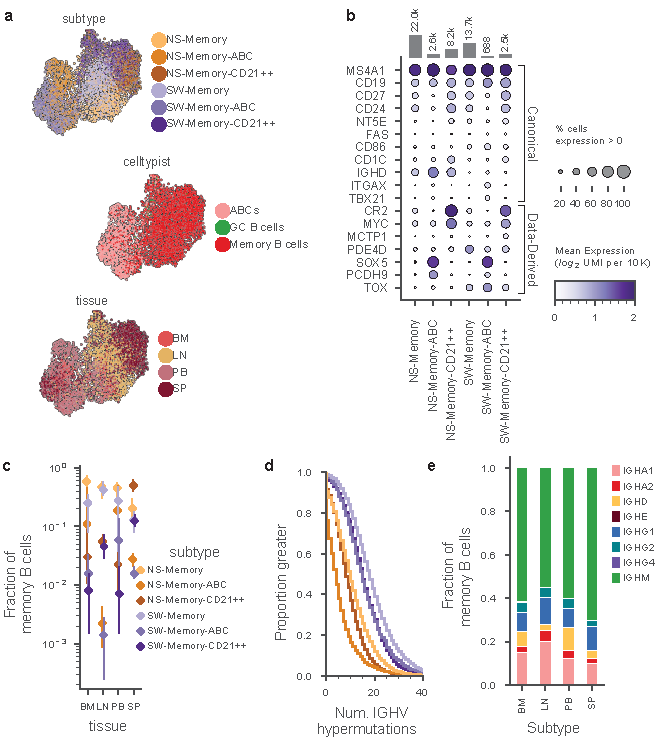
\includegraphics[width=12cm, keepaspectratio]{figs/Tabula_Bursa/EDFigure2_MemB_subtypes.pdf}
    \caption[Heterogeneity in memory B cells.] {(a) Low-dimensional (UMAP) representation of transcriptional heterogeneity in memory B cells. Celltypist labels (top), (middle) transcriptome-derived labels, and tissue (bottom). For these UMAPs, celltypes were sampled uniformly before calculating a neighbors graph. (b) Genes distinguishing between the subtypes of memory B cells, where the top half of the plot shows canonical genes often used for flow cytometry and the bottom shows the data-derived, transcriptionally detected genes which distinguish the subtypes. (c) The relative fractional abundance of memory B subtypes in tissues averaged across all donors. (d) The distribution of  hypermutation levels. (e) Barplot of constant region usage in tissues}
    \label{ED:memoryb-overview}
\end{figure}


\begin{figure}
    \centering
    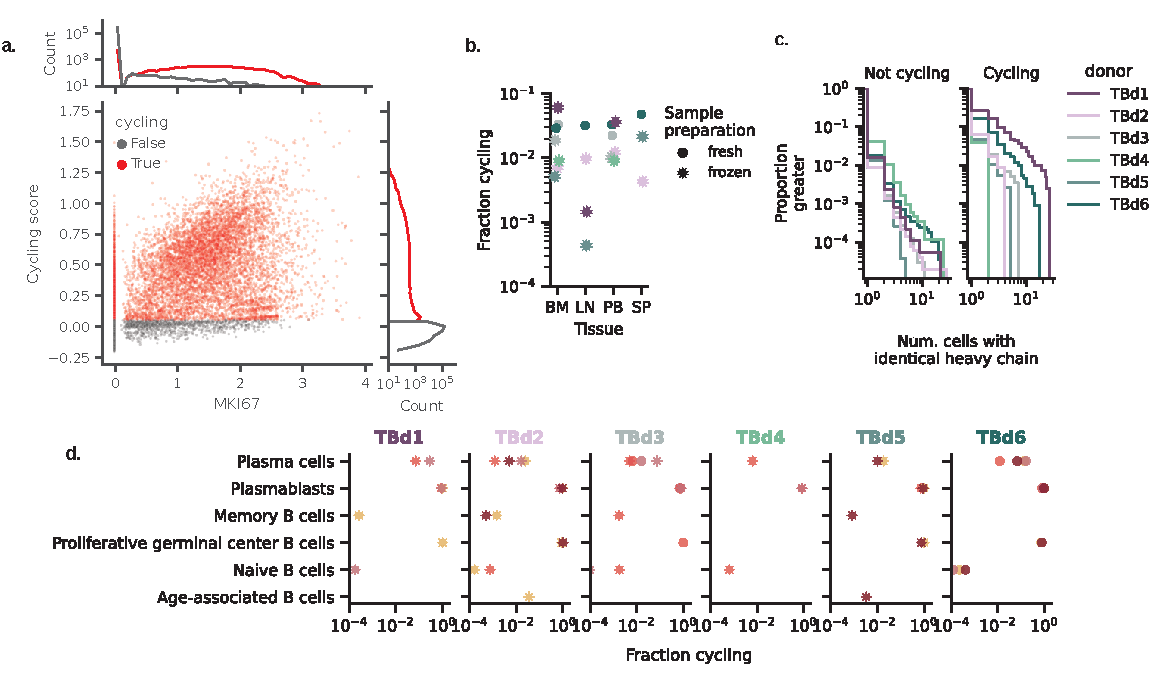
\includegraphics[width=10cm, keepaspectratio]{figs/Tabula_Bursa/EDFigure1.pdf}
    \caption[Cell cycle analysis across tissues.] {(a) Jointplot of the cycling score (calculated using the set of 30 genes most correlated with MKI67 expression) and normalized $log_2$ transcript counts of MKI67. (b) Fraction of cells cycling for each donor in each tissue. (c)The distribution of numbers of cells with identical VDJ sequences. (d) Fraction cycling shown for different celltypist defined cell types, with markers denoting fresh or frozen as in (b) }
\label{ED:cycling}
\end{figure}